\note{Detailed description of the subtasks that your system performs: 
how does it tackle these subtasks? 
why did you choose this approach? 
did you encounter specific problems that you had to solve? 
how did you solve them?}

\subsection{Data}\label{sec:data}
\subsubsection{Corpus Description}\label{sec:description_of_the_castro_archive}
\paragraph{Structure}
The \citeA{CastroDB} (CSDB) is an online corpus consisting of speeches, interviews, press conferences and other oratory by Fidel Castro from 1959 to 1996 translated into English, maintained by the Latin American Network Information Center (LANIC) at the University of Texas at Austin. The collection contains 1492 documents with an average document size of approximately 3,800 words. The information is presented as plain-text documents embedded into HTML web pages organized by the year and month of the original release. The documents are annotated with metadata including:

\begin{itemize}
\item The type of document (e.g.\ \scare{speech}, \scare{interview}, \scare{press conference})
\item The exact date of the original release
\item The author, e.g.\ Castro himself or a particular reporter
\item The original source, e.g.\ \scare{Havana Domestic Radio}
\item A headline (such as in a newspaper)
\item The reporting agency, e.g.\ the Foreign Broadcast Information Service (FBIS)
\item The exact date of the report
\end{itemize}

\paragraph{Linguistic properties}
The documents are manually translated from modern Spanish into modern English, sparing us many problems associated with documents written in historical languages. This characteristic, along with a considerable amount of newspaper comparable content allow a relatively straightforward application of technologies already deployed and currently used in NLP and IR.

However, the corpus is very heterogeneous: Not only does it span 37 years of oratory, but it also incorporates many different authors. Although it is a database dedicated to the oratory of Fidel Castro, it features many documents which are not narrated by Castro, for instance by news reporters, journalists and interviewers. Likewise, the corpus comprises many different genres and styles.

Secondly, many of the documents in the corpus are (at least indirectly) based on spoken language and so are not structured in a formal way, in polar opposition to e.g.\ a scientific report. Likewise, many documents in the corpus feature heavily-rhetorical content. Due to this characteristic, in many documents, topics are multiple and often vague. This observation is valid for the whole documents as well as smaller sections such as single paragraphs. 

In this way, the corpus is less similar to relatively-structured corpora (such as the Wall Street Journal-based \citeauthor{PTB}) it is to less-structured and more heterogeneous literary corpora. On these kinds of documents, topic identification as well as document summarization and clustering is difficult to implement manually (using human competence), let alone doing so automatically.

\subsubsection{Reading and Storing the Data}\label{sec:reading_and_storing_the_data}
\note{reading the data, creating MySQL database, creating data model}

At a first step we used a \texttt{shell}\footnote{http://tiswww.case.edu/php/chet/bash/bashtop.html}
script and \texttt{wget}\footnote{http://www.gnu.org/software/wget/} to download the complete castro
speech database. The actual speech data consists of a set of static webpages sorted by year into
folders. In a second processing step we parsed these html-files and extracted the actual content of
each file and its meta-information into textual format. To this end, several \texttt{shell} and
\texttt{python}\footnote{http://www.python.org/} scripts have been written.

The extracted information serves as the basis for the consecutive analysis and processing steps. In
order to provide structured access to the meta-information we developed a
\texttt{perl}\footnote{http://www.perl.org/} script to convert the meta-information for each
document into an entry in a \texttt{mysql}\footnote{http://www.mysql.de/products/enterprise/}
database. For every document, the database provides the following information
\begin{itemize}
 \item{\textsc{Author:} Name of the author of the document.}
 \item{\textsc{Location:} The place the document orginated.}
 \item{\textsc{Headline:} The headline of the document.}
 \item{\textsc{Date:} The date the document orginated.}
 \item{\textsc{ReportDate:} The date th3e content of the document appeared in written from.}
 \item{\textsc{Type:} There are several different types of documents in the databse. E.g.
 \texttt{SPEECH}, \texttt{INTERVIEW}, \texttt{ARTICLE}, etc.}
 \item{\textsc{Header:} Additional meta-information}
 \item{\textsc{Source:} The source where this document appeared in written form the first time.}
\end{itemize}
In addition to this information, we later enriched the database with the extracted named entities
(see \ref{sec:named_entity_recognition}) for each document. The columns \textsc{Persons},
\textsc{Places}, \textsc{Organizations} have been added and each field contains the bulk information
of the identified named entities as a comma separated list. Although this representation is is not
the most elegant and optimal solution, the derived database provides sufficient performance and
usability for the task at hand.

\subsection {Named Entity Recognition}
\label{sec:named_entity_recognition}
Please recall, that our ultimate goal is to come up with a cross-document recommendation system for
the castro speech database. Therefore, we need an appropriate metric on between document
similarity that serves as a basis for the recommendation software.

Our first idea was to use proper \textit{co-reference resolution}, e.g. provided by
\texttt{BART}\footnote{http://www.bart-coref.org/} software \cite{bart}. In this case, document
similarity is a function of the number of co-references that appear between two docuemnts. However,
in the end we decided to drop this approach because of the overall complexity and the tight time
constraints. In general, between document co-reference resolution far from an easy task. The castro
database though has some nice properties that allow for a more straightforward solution. For this
dataset, the domain is rather limited and the number of distinct topics should be small. Hence, we
came up with the idea to base the similarity measure on smoothed co-occurences of named entities.

The next step in the pre-processing chain is thus the execution of named entity recognition followed
by a smooting of the features in the vector space induced by the named entities using kernel
methods (see \ref{sec:string_kernel}) \cite{string_kernel_coref}.
\subsection{Named Entity Recognition}\label{sec:stanford_named_entity_recognizer}
\note{identifying names, locations and organizations in the Castro documents,
input/output examples, evaluation??}

YEVGENI WILL WRITE

CARSTEN - PROVIDE STATISTICS TABLE, WRITE ON TECHNICALITIES WITH RUNNING THE NER AND STORING RESULTS
\begin{figure}[ht]
\centering
\caption{Global statistics for the named entities. The table shows the number of distinct named
entities found by the stanford named entity recognizer and the average number of occurences for
each NE type per document.}
\begin{tabular}{l|ll}
  Named Entity Type      & Number & Average/Document\\
  \hline
  \textsc{Person}        & 6515   & 21.5\\
  \textsc{Organizations} & 3667   & 44.7\\
  \textsc{Locations}     & 6612   & 17.1\\
\end{tabular}
\label{fig:ne_statistics}
\end{figure}

For the subtask of named entity extraction we used the Stanford named entity recognizer (sNER)
\cite{sner} version $1.1.1$. The package provides several pre-trained classifiers trained on both US
and UK newswire data from CoNLL, MUC6, MUC7 and ACE.

The named entity recognition was performed with the
\texttt{ner-eng-ie.crf-3-all2008-distsim.ser.gz} model - a three class classifier for the named
entities \textsc{Person}, \textsc{Organizations} and \textsc{Locations} with an additional
``distributional similarity lexicon'' for improved performance. Processing was done by a
\texttt{shell} script that runs sNER for each document in the castro database. The input is a
textfile containing the content of a document without meta-information. For the output format we
choose a XML dialect.



\subsection{Representing Documents in Vector Space}\label{sec:representing_documents_in_vector_space}
MICHAL 

\subsubsection{Indexing}
\label{sec:indexing_term_weighting}
\note{description and motication of the 4 different representations}

\subsubsection{Term Weighting}
\label{sec:term_weighting}
\note{ tf/tfidf with motivation and
interpretation for each, examples}

Vector model is the model of representing text document or any other data. In vector model for information retrieval both documents and queries are represented as a vector of numbers. Number at each position of the vector corresponds to the term importance for the representation of the query or document. The main advantage of the vector model is that it has easy algebraic formulation. It's also not that strict as the boolean model. In boolean model document either completely fits to the query or it doesn't fit at all. In real word the situation is different, the relevance of the document for the user is rathed continuous quantity and the same applies to the vector model.

The coefficients are usually normalised in order to have the same length, otherwise the model would favor the documents with greater length. What is important is the density of the term in the document.

There are several measures beeing used which express the importance of the index term for the document. The most widely used are TF and TF-IDF. 
TF stands for term frequency, it measures directly how many times the word occured in the document, TF score grows linearly with the number of occurences of the term in the document. The TF score of term j in document i is defined as follows:

\note{Someone who can work with latex please add the following: $text{TF}(i,j) = n(i,j)$ / SUM(k
over all terms) n(i,k) }
\[\text{TF}(i,j) = n(i,j) / \sum_{k \in \mathcal{T}}{n(i,k)}\]

$n(i,j)$ stands for the number of counts term $j$ occured in document $i$.

TF-IDF stands for term frequency - inverse document frequency. This measure is based on the notion that the terms which occur in a lot of documents are not very useful for searching purposes. The terms which occur in a few documents only have greater discrimination power. The TF-IDF score of term j in document is is defined as follows.

\note{Someone who can work with latex please add the following: TF-IDF(i,j) = TF(i,j) * log( |D| /
\{d: t(j) "is member of sign" d\} }
\[\text{TF-IDF}(i,j) = \text{TF}(i,j)\log{(|D| |\lbrace d : t(j) \in d \rbrace|)}\]

The TF-IDF score of term j drops according to the logarithm of the number of document that contain term j. The TF-IDF score of the term which is contained in every single document is always equal to zero.

\note{The indexes in brackets should be written in foot-script, I hope you show me tomorrow how to write formulas:) }  

In vector model we need to measure the similarity between vectors. The similarity is usually expressed by the cosine similarity measure:

\note{ cosim(q,d) = [SUM(k over all terms) q(k) * d(k)] / [ |q| * |d| ] }
\[\text{cosim}(q,d) = \sum_{k \in \mathcal{T}}\frac{q(k)d(k)}{|q||d|}\]

It express the cosin angle between the vectors q and d. This measure is equal to 1 for the paralell vectors and it's equal to zero for the perpendicular vectors.

In vector model the searching proceeds as follows. The search query is transformed into its vector representation in the same manner as it is done for the document. The cosine similarity between the query vector and the vector representation of each document is computed. The search results are ordered according to their similarity to the user query.  

Vector representations of the documents are stored in the index matrix. Each row of the index matrix corresponds to the vector representation of a single document. 

Our model contains several index matrix. We created index matrix for each named entity type and also index matrix for general index which indexes the non named entity terms. For all named entity types aliased or non-aliased index matrix can be used. Our current implementation of vector model doesn't use TF-IDF measure for adjustment of query terms. It means that all the values corresponding to the search terms in the query are the same in the vector representation of the query. In the future we would like to implement proper TF-IDF weighting of the query terms. \note{Check whether the TF-IDF weighting of query terms is common praxis} We would also like to implement query expansion using the string kernel. In current implementation query term must match exatly the named entity in the database otherwise the search term is not taken into the account. String kernel expansion would allow us to match query named entity with the named entity stored in the index file even when they don't match perfectly. In the current version query terms which are named entities must also have the proper capitalization.

Document retrieval in our model consists of two steps. In the first step, document, that don't satisfy the condition concerning the type and date of the document, are filtered out. In the second step documents are sorted in descending order according to their cosine measure similarity with the query. Only the subset of the best results of the size specified by the user proceeds to the next stage.


\subsubsection {Aliasing with String Kernels}
\label{sec:aliasing_string_kernel}
\note{motivation, description of the algorithm to create similarity matrixes between NE's,
smoothing document representations with Kernel matrix as aliasing}



\subsection{Aliasing with String Kernels}\label{sec:aliasing}
In general, the idea of kernel methods is to map objects of a
distinct type $K$ into some \textit{Hilbert space} $\mathcal{H}$ using a mapping function $\Phi :
K \rightarrow \mathcal{H}$. Here, $K$ can have an arbitrary structure, e.g. trees, strings,
graphs, etc. Given such a mapping $\Phi$ the similarity of two objects $s,t \in K$ can be computed
by using the scalar product defined on the Hilbert space:
\[sim(s,t) = <\Phi(s),\Phi(t)>\]
Instead of defining the mapping function $\Phi$ explicitly, a kernel function $k : K \times K
\rightarrow \mathbb{R}$ can be used. Kernel functions are positive-semidefinite functions
who implicitly compute the scalar product of two objects on some Hilbert space. That is, for every
kernel function $k$ there exists a mapping $\Phi$, such that
\[k(s,t) = <\Phi(s),\Phi(t)>.\]
This property of kernel functions is often exploited in practice because it greatly facilitates the
computational cost that is needed to compute object similarity.

\textit{String kernels} are kernel methods \note{cite} that operate on the domain of strings over
a finite alphabet $\Sigma$ and are often applied in the fields of \textit{information
retrieval} and \textit{bioinformatics}. For the purpose of our work, we applied a
\textit{p-spectrum} string kernel \note{citation needed} which is defined by
\[k_p(s,t) = \sum_{u \in \Sigma^p}{\phi_u^p(s)\phi_u^p(t)},\]
where $\phi_u^p(s)$ counts the number of occurrences of the substring $u$ of length $p$ in $s$. The
associated Hilbert space for this kernel is $\mathbb{R}^{|\Sigma^p|}$ - the space of all possible
strings over $\Sigma$ of length $p$. The p-spectrum string kernel can be efficiently implemented by using \textit{trie} data-structures and \textit{n-gram} models.

\subsubsection{Co-reference Resolution by String Kernels}
\label{sec:co_reference_resolution_by_string_kernels}
Co-refernce resolution by kernel methods is an active research area and several methods have been proposed for the task. These include string and tree based kernel methods \cite{string_kernel_coref}.
The advantage of tree based methods is due to the possibilty to encode additional structure and information about syntactic and semantic properties of the text, which renders these methods superior to string based methods.

For our project, we only need co-reference resolution based on the extracted named entities. This essentially comes down to the task of \textit{aliasing} named entities for each type of named entity. To this end, we applied a two-spectrum string kernel. \note{explain this a little more}

\begin{figure}[ht]
  \caption{Example for aliasing of document- or query-vectors by string kernel similarity.
The matrix $\mathcal{S}$ is the \textit{kernel matrix} of the three terms $\mathcal{T} = \lbrace
\text{Fidel Castro},\text{Dr. Fidel Castro}, \text{Raul}\rbrace$. The first and second term have a
very high lexical similarity of $0.8$ while the third term is highly dissimilar. Using
$\mathcal{S}$, a document vector or query $q=(1,0,0)$ can now be expanded into an aliased form
$\bar q$, where $\bar q = \mathcal{S}q$. In general, aliasing is performed on all document vectors
and queries.}
  \[
     \underbrace{\begin{pmatrix}
      1   & 0.8 & 0\\
      0.8 & 1   & 0\\
      0   & 0   & 1\\
     \end{pmatrix}}_{\mathcal{S}}
     \underbrace{\begin{pmatrix}
     1\\ 0\\0 
     \end{pmatrix}}_{q}
     =
     \underbrace{\begin{pmatrix}
     1\\ 0.8\\0 
     \end{pmatrix}}_{\bar q}
  \]
  \label{eq:example_string_sim}
\end{figure}

\note{how we did coref}
\note{cpp implementation, simmatrix as sparse matrix... approximation...}

The first implementation of the two-spectrum kernel function was done in \texttt{python} but we  later reimplemented it in \textt{C++} for performance reasons. For all three types of named entities we computed the complete kernel matrix $\textbf{K}$, where $\textbf{K_{i,j}}$ is the similarity of the named entities $i$ and $j$. Since many of the entries in $\textbf{K}$ are near zero, thresholding with a fixed value was applied after the computation and the resulting sparse matrix was then stored.

Now given the kernel matrix $\textbf{K}$, aliasing can be performed through multiplication of each document-vector with the kernel matrix. The scalor prodact on the resulting aliased document vectors yields the overall document similarity with respect to the named entities. In figure \ref{eq:example_string_sim} we give a short example on aliasing based on three different named entities.





HOW IT RELATES TO FULL COREFF SESTEM, HOW IT RELATES TO OTHER STRING DISTANCE METHODS

IMPLEMENTATION ASPECTS (which package, additional scripting etc.. )

PROBLEMS, SOLUTIONS





\subsection{Information Retrieval}\label{sec:information_retrieval}
\subsubsection{Keyword Search}\label{sec:keyword_search}
\note{description of the functionality, use of string kernels for query expansion }

\subsubsection{Metadata Search}\label{sec:metadata_search}
\note{general description of the functionality}

\subsection{Computing Similarity between Documents}\label{sec:computing_similarity_between_documents}
\input{documentsimilarity}

\subsection{Graphical Representation}\label{sec:graphical_representation}
\subsubsection{Computing Graph Layouts}
So far we have described how nodes and edges of the graph are obtained from documents and their
similarity. In order to display the graph, a graph layout (two dimensional representation of the
graph) must be determined. If the vector representation of the document is only two dimensional,
then it is straightforward to obtain the graph layout just by using the features as two dimensional
coordinates. However, the documents in our model are represented by vectors with several thousands
of dimensions. The problem of reducing the dimensionality, is usually not solved by mapping
from high dimensional vector space to the low dimensional vector space but by using algorithms that
solve the problem of graph layouting directly using only the properties of the underlying graph
(nodes and edges together with their weights).

The layouting algorithm that was used in this project belongs to the popular class of force-based
layout algorithms which are based on physical modeling. An Edge is considered a spring and
the nodes are considered to be electrically charged particles (i.e.\ with equal signed charge such
that they repel each other) The optimal length of the springs is set in advance. Springs whose
length is larger or smaller than their optimal length exert a force that acts on the connected
nodes. In each iteration of the layouting algorithm, nodes are moved according to the resultant
force
that acts on them. After some time the position of the nodes becomes (quasi) stationary and the
system get into a local equilibrium state.

The described class of force based layout algorithms subsumes various algorithms with different
properties. However, they all perform variations of force-field energy minimization by iterative
approximation schemes. In this project the very basic algorithm as it is described in the previous
paragraph was used.

\subsubsection{Jung Graph Framework}
For the purpose of graph layouting, graph painting and user-graph interaction, the
\texttt{Jung\footnotemark{http://jung.sourceforge.net/} - java universal network/graph framework}
was used. It provides great flexibility in adjusting the graph appearance. Several so-called
transformers which affect node and edge label appearance can be plugged together to result in the
aesthetically pleasant appearance. \texttt{Jung} also provides predefined classes that allow for
easy interaction with the user. Functionalities for graph translation, zooming, node selection, node
transposition and other features can be achieved with minimal programming effort. One notably
strong point of the library is its template based design with the possibility to include several
plug-in components such as rendering and transformers that affect the resulting appearance of the
graph.

However there are some aspects of the \texttt{Jung} library, that were annoying fro the project.
First, it is difficult to achieve certain low level functionalities, like e.g.\ monitoring the
on-screen position of a fixed point while translation of the graph was performed. Secondly, several
operation are implemented in a circumstantial way. For example, in order to change the color of
one node the whole graph must be redrawn and during this process all active visualization
transformers are applied on each graph object.When we used the default implementation of the
\texttt{Jung} visualization class, the application consumed more then 50\% of the processor time
even though there was no ongoing user interaction or computation task (this depended on the size of
the presented graph --- the statement holds for graph with 25 nodes about 50 edges). By extending
the standard \texttt{Jung VisualizationViewer} class and overriding several functions, the issue of
unnecessary graph redrawing was resolved and accordingly the problem of the low gui performance.

\subsubsection {Querying Functionalities}
\label{sec:querying_functionalities}
The nodes of the graph are generated from the results of a database query supplied by the user, who
can search either by keyword, by NE, or by a combination of both in the same query. Likewise, the
user may select a range of years to search in (e.g.\ retrieve documents occurring between
\code{1970} and \code{1975}), as well as select only certain types of documents to be searched
(e.g.\ retrieve only documents of type \meta{Speech} or \meta{Interview}). The documents most
relevant to the current query are displayed, the number of the documents displayed being specified
by the user (e.g.\ display the \code{25} most relevant documents), and edges connecting each
document are drawn based on the similarity measures relating each document to each other.

\subsubsection {Presenting Results}
\label{sec:presenting_results}
After submitting a query, a table of query results is displayed and a graph corresponding to the
results is drawn, in which the relevance measure of each document to the current query is
represented by the absolute size of the node representing the document in question: The larger the
node, the more relevant it is to the current query. The type of document represented by the node is
represented by its shape, e.g.\ \meta{Speech} $\rightarrow$ star, \meta{Meeting} $\rightarrow$
pentagon. The edges linking the nodes of the graph represent the strength of similarity the of the
two documents represented by the nodes.
	
\subsection{Combining It All: User Interface}\label{sec:combining_it_all:_user_interface}
The query functions, graph and display functions are integrated into a single graphical front-end relying primarily on the mouse for user input. The graph representation is dynamic and interactive, able to be navigated through by the user in order to obtain detailed information regarding the document database.

\begin{figure}[ht]
\centering
\caption{GUI}
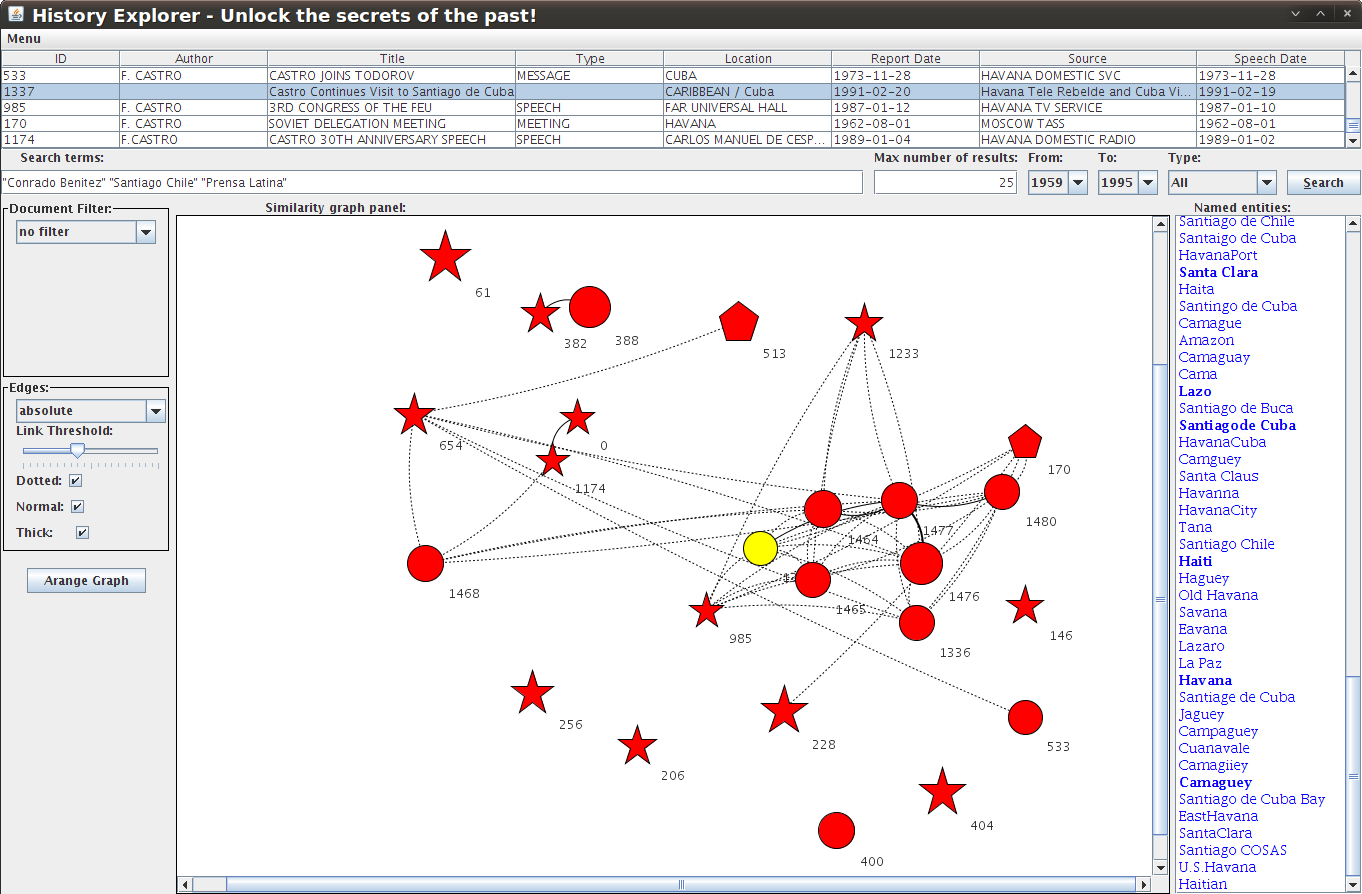
\includegraphics[width=160mm]{gui.png}
\end{figure}

\subsubsection{Search Function}
\begin{figure}[ht]
\centering
\caption{Search query}
\subfloat[][~\hfill{\tiny Version $<$\code{2010-04-02}}]{
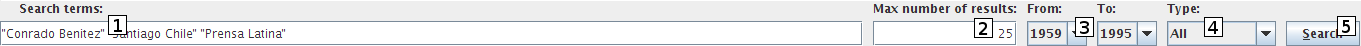
\includegraphics[width=160mm]{search.png}
}
\end{figure}

Search terms are entered in the query form (item 1 in the figure above)\footnote{Unless otherwise mentioned, the version depicted is \code{2010-04-02}.}: Entering any term will return both NEs and also keywords sharing the exact form (not case-sensitive)--- For instance, entering \lingform{committee} will both return exact instances of \code{committee} in the document itself, and will return NEs similar to \lingform{committee} based on the string kernel similarity measure, e.g.\ \lingform{Central Committee} and \lingform{Central Committee of the Cuban Communist Party}. Multi-word terms are denoted in double quotes, e.g.\ \code{"Central Committee"}. The maximum amount of query results can be adjusted (item 2): For example, entering a value of \code{10} will return ten documents most relevant to the query. The set of years searched between is also modifiable specified by (item 3), as well as the type(s) of documents searched (e.g.\ \code{Speech}, \code{Interview}) (item 5). Once the criteria are entered, the query is run by selecting item 5.

\paragraph{Presentation}
The results of the current query are displayed both in a table of results and in a graph displayed in the main window.

\subsubsection{Visualization of Results}
\begin{figure}[ht]
\centering
\caption{Query Results Table}
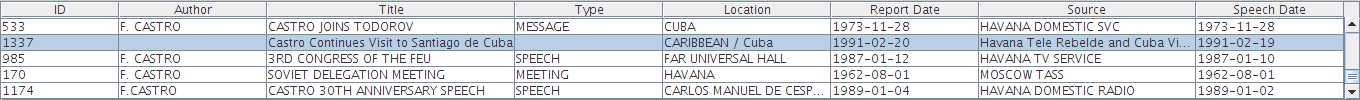
\includegraphics[width=160mm]{table.png}
\end{figure}

In the table, the documents are displayed in rows sorted by their relevance to the query in descending order. The metadata associated with each document is displayed in columns. If there was no metadata retrieved for a document, the entry for the data is empty or \code{NULL}.

\begin{figure}[ht]
\centering
\caption{Document Similarity Graph}
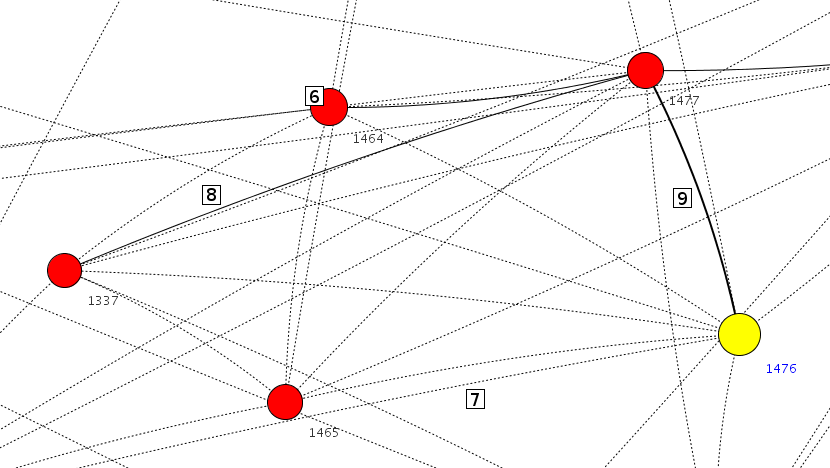
\includegraphics[width=80mm]{nodecloseup.png}
\end{figure}

In the graph, each document is represented by a node (item 6). The relevance of the document to the query is represented by the size of the node: The larger the node, the more relevant the document is to the submitted query. The edges between the nodes represent similarities between the documents based on the similarity of the two documents based on the NEs each contain and their aliases according to the string kernel measure. The stronger the similarity connection, the heavier the line weight of the edge drawn. There are three line weights: ``dotted'' (item 7), ``normal'' (item 8) and ``heavy'' (item 9), in ascending order of the level of similarity they represent. The graph can be scaled in real-time by zooming in and out with the scroll wheel. Furthermore, it is able to re-arrange the position of each node in the graph by clicking and dragging them in order to optimize the view of the graph manually. The graph can also be set to re-arrange the nodes automatically by clicking ``Arrange Graph''. By pressing CTRL and clicking on a node, the view will be centered on the said node automatically.

\paragraph{Navigation}
Selecting a document either through its corresponding entry in the table or node in the graph with the mouse or keyboard highlights it and displays the NEs in the document in a sidebar. The NEs in a particular document and their string kernel-based aliases are displayed in the sidebar: Boldface entries represent NEs in the given document, while the non-boldface entries represent NEs similar to the boldface NEs in the document according to the string kernel similarity measure. For example, the NE \textbf{\lingform{Castro}} may also return the similar NEs \lingform{Fidel}, \lingform{Fidel Castro} and \lingform{Dr.\ Fidel}. The type of the NE (e.g.\ \meta{person} or \meta{organization}) is represented by the color of the text, e.g.\ red for \meta{Persons}, green for \meta{Organizations} and blue for \meta{Locations}. It also is possible to select multiple documents, e.g.\ by holding SHIFT and clicking on multiple nodes/table entries, or by clicking and dragging the mouse to create a selection box encompassing the nodes/table entries to be selected. When multiple documents are selected, the entries displayed in the sidebar are those that are common to all selected documents.

\begin{figure}[ht]
\centering
\caption{Node Context Menu}
\subfloat[][~\hfill{\tiny Version $<$\code{2010-04-02}}]{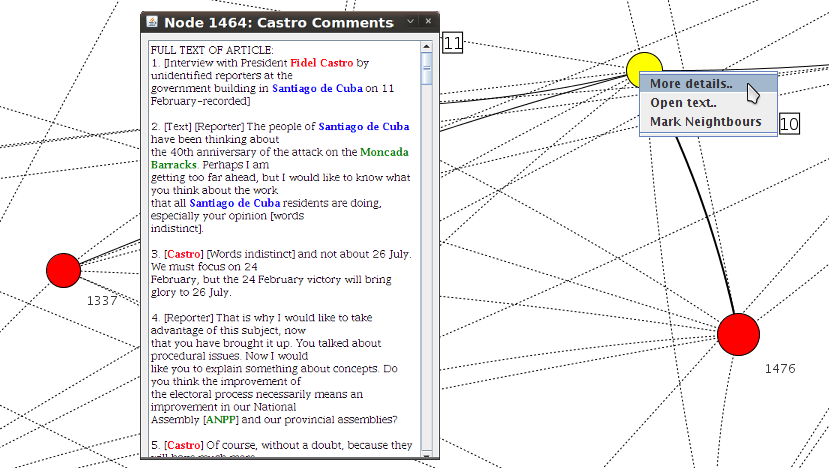
\includegraphics[width=80mm]{nodeclick.png}}
\end{figure}

In addition to viewing document metadata in the query results table, the user may to view the metadata of the document associated with a particular node (e.g.\ document \meta{Type}, \meta{Date} or \meta{Location}) through the node's context menu (item 10) (i.e.\ by right-clicking on the node with the mouse). Also available through the context menu is the text of the document itself, which is displayed in a separate window which can be kept open while still navigating through the graph and viewing other nodes (item 11). The NEs in the text are denoted by being colored according to their type.

\paragraph{\scare{Mark Nearest Neighbors} Function}
Lastly, it is possible through the context menu to automatically select the nearest neighbors of the selected node(s), i.e.\ to select the nodes which share a NE directly with the said node.

\begin{figure}[ht]
\centering
\caption{\scare{Mark Nearest Neighbors} Function}
\subfloat[][Before]{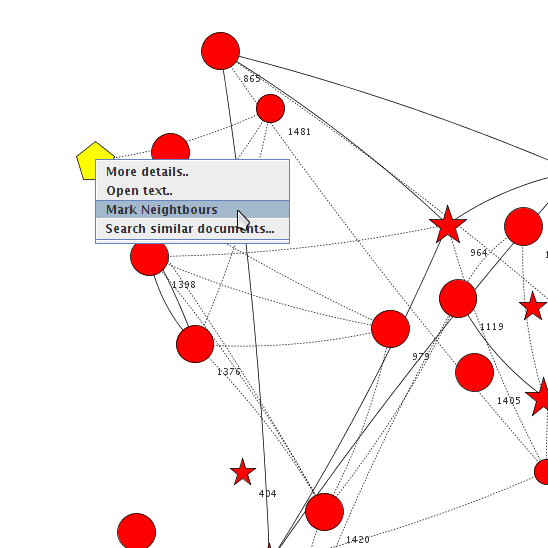
\includegraphics[width=80mm]{markneighbors_before.png}}
\subfloat[][After]{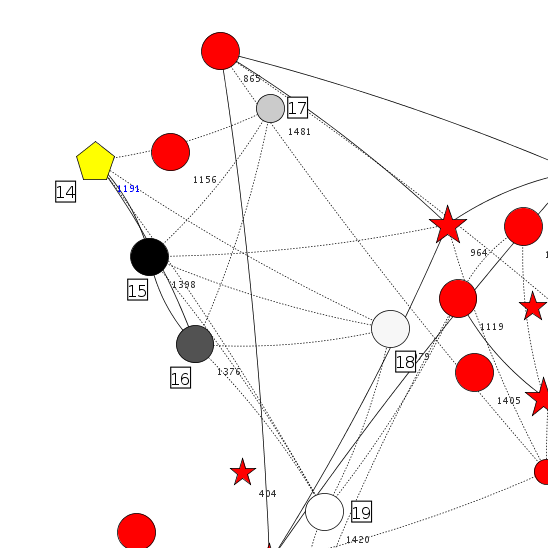
\includegraphics[width=80mm]{markneighbors_after.png}}
\end{figure}

Each nearest neighbor is automatically shaded in a range from black to white to represent the level of similarity between the node and the originally-selected node (item 14): The darker the shade, the more similar the document is to the document of the originally-selected node in relation to the other nearest neighbors; The lighter the shade, the less similar the document is. For example, of the nearest neighbours, item 15 is most similar to the originally-selected node. In descending order of similarity, the next most similar documents are item 16, 17 18 and 19.

\paragraph{Display Options}
\subparagraph{Edge/Node Filtering}

\begin{figure}[ht]
\centering
\caption{Display Options}
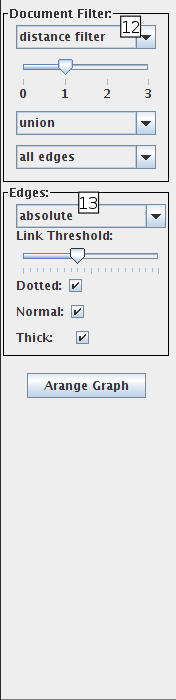
\includegraphics[height=80mm]{displayopts.png}
\end{figure}

The graphical display may be further adjusted by applying a distance filter (item 12) or by adjusting the method by which edges are drawn (item 13).

By default, the edges drawn are determined by the absolute similarity measure: If the similarity measure of two documents is greater than a user-adjustable edge threshold, an edge is drawn between them. The higher the absolute similarity of the two documents, the thicker the edge. However, the user may set the method of edge generation to display edges according to the relative similarity of the documents shown: According to the user-specifiable edge density, the more similar two documents are compared to the similarities of other documents, the thicker the edge.

By adjusting the edge threshold (for absolute similarity) or the edge density (for relative similarity) the user can adjust the level of detail represented by the graph. This allows the user to both discern relationships between documents which are not very similar to each other, and to prune out relatively weaker relationships between documents which are very similar to each other.

Likewise, a vertex filter may be applied, enabling the user to display only nodes of a specified distance $\leq x$ from a selected node or nodes, e.g.\ displaying only the nodes directly connected to the current node(s) (a distance of 1) or displaying nodes which are connected to the selected node through at most one other node (a distance of 2). When selecting multiple nodes, the user can select to display either the union of the neighbors, e.g.\ to display the nodes with a distance of $\leq x$ from \emph{any} selected node, or the intersection of the neighbors, e.g.\ to display only the nodes with a distance of $\leq x$ to \emph{all} selected nodes.

This may be done in real-time, i.e.\ after applying a distance filter, the user may select a node in the graph to view an updated graph of all nodes satisfying the distance criterion for the newly-selected node. This feature allows the user to explore ``sub-graphs'' of the main graph in real-time, allowing the user to focus on a particular cluster of documents and thus allowing the user even greater control over the search results.

\subparagraph{Advanced Options}
Finally, for even further control, the user may manually specify all display settings through the \scare{Setup} menu.

\begin{figure}[ht]
\centering
\caption{Advanced Settings}
\subfloat[][]{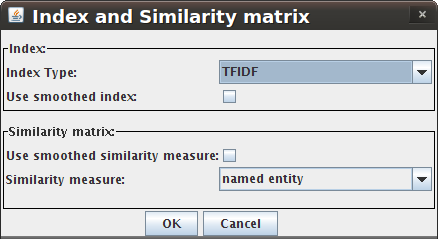
\includegraphics[scale=0.33]{menu_matrices.png}}\quad
\subfloat[][]{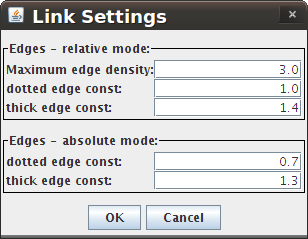
\includegraphics[scale=0.33]{menu_links.png}}\quad
\subfloat[][]{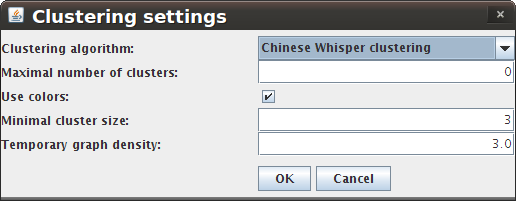
\includegraphics[scale=0.33]{menu_clustering.png}}
\end{figure}

\begin{description}
\item[\scare{Index and Similarity Matrix}] \hfill \\
The user can choose to have document similarities calculated with TF/IDF measures (default) or simply TF scores. Additionally, similarities may be calculated with aliasing through the string kernel, or to calculate document similarities with aliasing disabled and associating only exact strings (default). Finally, the similarities can be calculated using only NEs (default), only lexical similarity, or may manually specify the weighting of each measure individually (\scare{custom}), e.g.\ of each type of NE compared to each other and to overall lexical similarity. 
\item[\scare{Link Settings}]\hfill \\
The edge density slider on the left-hand control panel left corresponds to the edge density value in relative-similarity mode, or the edge threshold value in absolute-similarity mode. When the graph is constructed in the relative similarity mode, the number of edges is determined by multiplying the number of nodes by the the chosen edge density (slider value), and the strongest edges are displayed according to this value. After the set of edges is determined, the mean of the edge strength is computed. The strength of each edge is then compared with the mean of the edge strength. The ratio between the edge strength and the mean of the edge strength determines whether the edge will be dotted, normal or thick.

\begin{itemize}
\item \scare{Maximum edge density}: determines which density value corresponds to the right corner position of the density slider.

\item \scare{Dotted edge const}: If the edge strength is lower than the mean of the edge strength multiplied by dotted edge constant, then the edge is dotted.

\item \scare{Thick edge const} If the edge strength is higher then the mean of the edge strength multiplied by thick edge constant, then the edge is thick.
\end{itemize}

The following settings control the edge appearance in absolute-similarity mode:

\begin{itemize}
\item \scare{Dotted edge const}: If the strength of the edge lies between the dotted edge threshold and the normal edge threshold, then the edge is dotted.
\item \scare{Thick edge const}: If the strength of the edge is greater than the thick edge threshold, then the edge is thick.
\end{itemize}

If the strength of the edge lies between the normal edge threshold and the thick edge threshold, then the edge is normal.

The threshold value for normal edges is determined by the slider in the main control panel. The dotted-edge threshold value is then computed as a product of the normal edge threshold and the dotted edge constant. Likewise, the thick-edge threshold value is computed as a product of the normal edge threshold and the thick edge constant.
\item[\scare{Clustering Settings}] \hfill \\
The user can enable Chinese Whispering (CW) automatic document clustering (disabled by default), and specify the maximum number of clusters formed, the minimum size of each cluster, as well as the temporary graph density. Temporary graph is the data structure that is used for computation of the clusters. For the purpose of the clustering algorithm it's better to have dense graph, while users prefer rather sparser graph. That's the reason why there is a temporary graph structure for the purpose of the clustering algorithm. 
Clustering can be enabled by setting the maximum number of clusters to the positive value.
We implemented a modified version of Chinese Whispering algorithm. Modified algorithm is less overgenerating. It puts the document to the cluster only when there is a strong evidence. By increasing the "Activation threshold multiplier" and by decreasing the "Init iterations" algorithm becomes more conservative and vice versa. 
\end{description}

All of these features combine to create a powerful interface for searching the corpus and visualizing the results which is both highly automated and highly customizable. In turn, the system is designed to accommodate both basic and advanced users.

